% !TeX root = ../Book1.tex
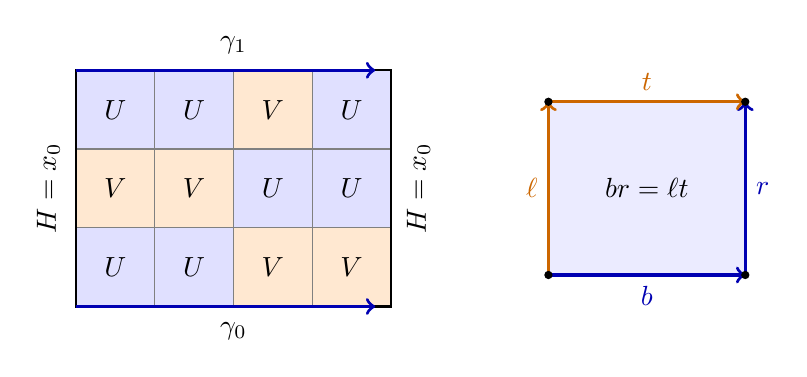
\begin{tikzpicture}[x=1cm,y=1cm]
	\foreach \x/\y in {0/0,1/0,2/1,3/1,0/2,1/2,3/2}{
		\fill[blue!12] (\x,\y) rectangle +(1,1);
	}
	\foreach \x/\y in {2/0,3/0,0/1,1/1,2/2}{
		\fill[orange!18] (\x,\y) rectangle +(1,1);
	}
	\draw[step=1,gray] (0,0) grid (4,3);
	\draw[thick] (0,0) rectangle (4,3);
	\foreach \x/\y/\s in {.5/.5/U,1.5/.5/U,2.5/.5/V,3.5/.5/V,.5/1.5/V,1.5/1.5/V,2.5/1.5/U,3.5/1.5/U,.5/2.5/U,1.5/2.5/U,2.5/2.5/V,3.5/2.5/U}{
		\node at (\x,\y) {\(\s\)};
	}
	\draw[very thick,->,blue!70!black] (0,0)--(3.8,0);
	\draw[very thick,->,blue!70!black] (0,3)--(3.8,3);
	\node[below] at (2,-.08) {\(\gamma_0\)};
	\node[above] at (2,3.08) {\(\gamma_1\)};
	\node[rotate=90] at (-.35,1.5) {\(H=x_0\)};
	\node[rotate=90] at (4.35,1.5) {\(H=x_0\)};
	\fill[blue!8] (6,.4) rectangle (8.5,2.6);
	\draw[very thick,blue!70!black,->] (6,.4)--(8.5,.4) node[midway,below] {\(b\)};
	\draw[very thick,blue!70!black,->] (8.5,.4)--(8.5,2.6) node[midway,right] {\(r\)};
	\draw[very thick,orange!80!black,->] (6,.4)--(6,2.6) node[midway,left] {\(\ell\)};
	\draw[very thick,orange!80!black,->] (6,2.6)--(8.5,2.6) node[midway,above] {\(t\)};
	\node at (7.25,1.5) {\(br=\ell t\)};
	\foreach \x/\y in {6/.4,8.5/.4,6/2.6,8.5/2.6}{
		\fill (\x,\y) circle (1.5pt);
	}
\end{tikzpicture}
